\chapter{The Chain \small{\textsf{DRAFT}}}\label{chapter:chain}

In the last chapter, we discussed the necessity for blocks as a mechanism to enforce \emph{periods of silence} so that double spends
can be adequately separated in time.  We then linked blocks together into chains in order to ensure freshness so that an adversary cannot
retroactively bring blocks mined and withheld in the old past. However, we left the notion of ``freshness'' and block validation
undefined. In this chapter, we will fill in all the missing details of how blocks and chains are verified. By the end of this chapter,
we will have a rudimentary, yet complete and secure, blockchain protocol.

\section{The Target}

Previously, we designed the proof-of-work inequality $H(B) \leq T$ in order to create \emph{rare events} and \emph{periods of silence}
as a moderately hard version of the exponentially hard hash preimage problem. In order to prevent double spends, we needed to ensure
that blocks are spaced $\Delta$ apart. Let us now calculate the correct value of $T$ so that block production is spaced more than
$\Delta$ time apart. To do this, we need to first find out when the proof-of-work inequality holds. If we start
with a freshly generated $\ctr$ and place it into $B = s \conc \overline{x} \conc \ctr$, what is the probability that $H(B) \leq T$?
This question is not straightforward to answer, because the output of a hash function may not be uniformly distributed (see also
Problem~\ref{problem:small-hash}).

In fact, not all collision resistant hash functions are suitable for proof-of-work. We want to demand that, whenever the hash is queried with a fresh input, the output is uniformly distributed in $\{0,1\}^\kappa$. This extra assumption is known as the \emph{random oracle model} and we will return to it in Chapter~\ref{chapter:earnest1}. Using the random oracle model, we can calculate the probability that a particular nonce trial is successful:

\glsxtrnewsymbol[description={successful query probability}]{successful query probability}{$p$}\glsadd{successful query probability}
\[
  p = \Pr[H(B) \leq T] = \frac{T}{2^\kappa}
\]

During the exhaustive search of proof-of-work, if a particular hash trial $H(B)$ is found to be $H(B) \leq T$, we call that hash function query a \emph{successful query}\index{Successful query}. Otherwise, if $H(B) > T$, we call the query \emph{unsuccessful}. The expected number of queries needed until a successful query is found is $\frac{1}{p} = \frac{2^\kappa}{T}$.

As protocol designers, we need to set $T$ correctly so that blocks are produced at a rate smaller than once per $\Delta$. For this, we need to have an estimate of how fast the participating nodes on the network can compute hash queries. Let's start with some definitions. Suppose that a typical honest computer can process
\glsxtrnewsymbol[description={compute}]{compute}{$q$}\glsadd{compute}
$q \in \mathbb{N}$
computations of $H$ during every unit of time. Let us also suppose that the total number of computers mining on the network is
\glsxtrnewsymbol[description={total parties}]{total parties}{$n$}\glsadd{total parties}
$n \in \mathbb{N}$
and the adversary controls
\glsxtrnewsymbol[description={adversarial parties}]{adversarial parties}{$t$}\glsadd{adversarial parties}
$t \in \mathbb{N}$
of them. Here, we are assuming that all computers have equal processing power, but if there is some computer on the network that has more processing power, we can just think about that powerful computer as a collection of smaller, less powerful computers, each of which has $q$ computational power. The model still works out. We will call each of these computers a
\emph{party}\index{Party}.
Each mining party will roughly correspond to a node on the network, but in practice these are not necessarily the same: A single network node can correspond to multiple parties if it is a powerful computer. On the other hand, because our system is permissionless, a party may spawn multiple nodes that all share the same computational power. Additionally, even though we are saying that the adversary is in control of $t$ adversarial parties, we are still considering the situation where the adversary is a ``puppet master'' who controls every adversarial party of the network by a central ``master plan'' $\mathcal{A}$. We say that such a party controlled by the adversary is \emph{adversarial}, \emph{corrupt}, or \emph{malicious}, and we will use these terms interchangably.

The total number of hash queries that can be executed in the unit of time is $nq$.
Since all parties are simultaneously trying to get a block all the time, the expected block generation
time is $\frac{1}{pnq} = \frac{2^\kappa}{Tnq}$. If we want this value to be above $\Delta$ we must demand

\[
  \frac{2^\kappa}{Tnq} > \Delta \Rightarrow T < \frac{2^\kappa}{nq\Delta}\,.
\]

In a nutshell, the more computational power there is on the network, the larger we must make the difficulty.
Also, the larger the network delay, the larger we must make the difficulty.

\section{The Arrow of Time}

In the previous chapter, we decided to link blocks together into a chain in order to ensure each block
has \emph{freshness} and cannot be brought back from the past. It turns out that this natural and
intuitive chain structure actually has many more nice properties than just ensuring freshness, which
we will explore over the next few chapters.

In order to be able to speak about chains more precisely,
let us introduce a bit of notation. A chain $\chain$ is a finite sequence of blocks
$\chain = (B_0, B_1, B_2, \ldots, B_{n-1})$ ordered chronologically.
The chain \emph{length} $|\chain|$ is the number of blocks in the chain.
We address these blocks by their zero-based index,
so $\chain[0]$ is the first (and oldest) block on the chain, $\chain[1]$ is the second, and so on.
The first block among a complete chain is the genesis block, so $\chain[0] = \mathcal{G}$.
We use negative indexing to address blocks from the end of the chain, so $\chain[-1]$
is the last (and most recent) block, $\chain[-2]$ is the penultimate block, and so on.
The block $\chain[-1]$ is called the \emph{tip}.
The index of a block within its chain is called the block's \emph{height},
so genesis has height $0$ and the tip has height $|\chain| - 1$.
It will also be useful to speak about \emph{chunks} of a chain, continuous portions
of the chain. We'll denote by $\chain[i{:}j]$ the portion of the chain starting at block
with index $i$ (inclusive) and ending at block with index $j$ (exclusive). For example,
$(B_0, B_1, B_2)[0:2] = (B_0, B_1)$. These $i$ and $j$ can also be negative, again meaning
indexing from the end. Omitting $i$ means starting from the beginning, while
omitting $j$ means going until the end of the chain. For example
$(B_0, B_1, B_2, B_3, B_4, B_5)[-2:] = (B_4, B_5)$.

We have not yet specified how to actually verify a block, and what are the conditions for
accepting a block. How exactly do we determine if a block is \emph{fresh} or \emph{unfresh}? Let
us try the following strategy to see where it leads.

\begin{quote}
A fresh block must extend the most recent block we've seen. If we receive a fresh block, we accept
it. Otherwise we reject it as unfresh.
\end{quote}

Having considered the simple ideas that don't work for transaction ordering, this strategy
seems eerily fragile. Let us go over an example where it breaks. Consider the
successful queries illustrated in the timeline of
Figure~\ref{fig.regular-adv-honest-queries}. In this timeline, the successful queries are spaced
apart more than $\Delta$ by an appropriate choice of the $T$ parameter. Some of the queries happen
to be honest (black solid diamonds), whereas other queries happen to be adversarial (red hollow circles).
The honest party who performed the successful query $1$ will mine a block on top of $\mathcal{G}$,
and broadcast it to everyone. Let's call this honest party \emph{party $1$} and the block just generated
\emph{block $1$}. Since block $1$ will reach the whole network by time $\Delta$,
everyone will have adopted it prior to the next successful query. Honest party $2$ will then
mine a block on top of $1$ and broadcast it to everyone, and so on, until the adversary gets
the successful query $5$. At this point, the adversary mines block $5$ on top of $4$, but can choose
to selectively disclose it. The adversary does \emph{not} disclose block $5$ to party $6$,
but discloses it to party $7$ at some time $t_A$ right before query $6$ occurs. Since $t_A$ and
query $6$ are less than $\Delta$ apart, party $6$ will not receive block $5$ before mining block $6$,
and so block $6$ will extend block $4$. At a later time $t_B$, occurring after query $6$ but before query $7$,
party $6$ receives block $5$, but
it is too late: He has already mined block $6$ and cannot go back and change it.
On the contrary, party $7$ has seen block $5$ prior to block $6$ and is made to falsely believe
that party $6$ wrongly chose not to extend block $5$. Party $7$ rejects block $6$ as \emph{unfresh}
and mines block $7$ on top of block $5$.

\begin{figure}[h]
    \centering
    \includegraphics[width=0.4 \columnwidth,keepaspectratio]{figures/regular-adv-honest-queries.pdf}
    \caption{A series of successful honest (black solid diamonds) and adversarial (red hollow circles) queries
             regularly spaced apart more than $\Delta$.}
    \label{fig.regular-adv-honest-queries}
\end{figure}

This scenario leads to the \emph{blocktree}\index{Blocktree} illustrated in Figure~\ref{fig.chain-fork}.
Worse yet, now some parties who detected that $5$ was broadcast late will accept $6$ as valid, whereas
the parties who received $5$ early will accept $7$ as valid. While we were hoping that the proof-of-work
construction would give us a single chain as a global source of truth, we have failed, and, again,
we have honest views in disagreement.

% TODO: add the network timeline of parties 6 and 7 to illustrate how messages were received
\begin{figure}[h]
    \centering
    \includegraphics[width=0.4 \columnwidth,keepaspectratio]{figures/chain-fork.pdf}
    \caption{A block\emph{tree} instead of a block\emph{chain} arising out of the timeline
             of Figure~\ref{fig.regular-adv-honest-queries}.}
    \label{fig.chain-fork}
\end{figure}

There is a disagreement about what is fresh and what is unfresh. We need to adopt a more
robust measure of time. Towards this, let us reinspect the chain structure we discovered
in the previous chapter.

Because the hash of a block cannot be predicted prior to the proof-of-work actually taking place
(otherwise proof-of-work would be solvable by a faster algorithm than exhaustive search),
the value
$s$ of the previd must be computed prior to the value $H(s \concat \overline{x} \concat \ctr)$.
In other words, the previd $s$ must already be known when mining for a new block that includes
$s$ as its previd. Blocks are mined in the order they appear. The pointers between blocks
in the chain are \emph{causality links}. They point backwards in time. The blockchain grows
forward in time and defines an \emph{arrow of time}\index{Arrow of Time}. When we observe a blockchain, we can
deduce that all of its blocks were mined one after the other in the order that we observe
them. In fact, if we have a blockchain consisting of a sequence of blocks, if we change
the payload $\overline{x}$ in an earlier block, this will cause the proof-of-work in that
same block and all subsequent blocks to become invalid: Changing the $\overline{x}$ of the
block will cause its own blockid to change and its proof-of-work to be invalidated. This, in
turn, requires changing the previd $s$ of the next block to maintain the chain structure,
causing \emph{its} proof-of-work to
be invalidated, and so on and so forth for every subsequent block on the chain. To change
the contents of one block of the chain, the adversary would have to go back and redo all
the proof of work. Hence, if the adversary cannot detach a block from its parent and append
it to a different parent to make it appear newer than it is.

A longer blockchain takes more time to generate, whereas a shorter blockchain takes less time
to generate (we will prove this relationship between blockchains and time precisely in
Chapter~\ref{chapter:earnest3}). Therefore, we can use the \emph{length} of a blockchain
to estimate how much time it took to generate, and how fresh its tip is.

This allows a more objective comparison about which chain to adopt. Since a longer chain takes
more time to produce than a shorter chain, its tip is roughly the ``freshest''.
We now adopt the following rule for which chain to choose among multiple candidate
chains:

\begin{quote}\index{Longest Chain Rule}
    \textbf{Longest Chain Rule. }
    Among all chains on the network, adopt the \emph{longest} chain (the one with the most
    blocks) as your \emph{canonical chain}\index{Canonical Chain}. If there are multiple
    competing chains of the same length, choose any chain arbitrarily.
\end{quote}

Using this rule, a node doesn't have to stay online on the network all the time to observe
which block is fresh and which one isn't. Additionally, two honest nodes that have seen the
same network messages, regardless of the order in which they received them, agree on their
verdict of which chain is best.

We can now summarize the honest miner's rules, which every honest miner is constantly running:

\begin{enumerate}
  \item Maintain a local canonical chain $\mathcal{C}$.
  \item Keep mining on the canonical chain.
  \item If mining is successful, broadcast the new block to the network, and update the local canonical chain.
  \item If not, keep mining.
  \item In the meantime, when a new valid chain arrives on the network,
        check its length, and update the local canonical chain if the
        newly arriving chain is longer than the existing canonical chain.
\end{enumerate}

Once a party has adopted a canonical chain, reporting a ledger of transactions
to implement the \emph{read} operation of a full node is straightforward:
Given an adopted chain $\chain = (B_0, B_1, \ldots, B_{n-1})$, the ledger reported is

\[
    L = B_0.\overline{x} \conc B_1.\overline{x} \conc \ldots \conc B_{n-1}.\overline{x}\,.
\]

Here, we use the notation $B.\overline{x}$ to denote the $\overline{x}$ component
of block $B$. The ledger reading rule tells us that we take the transactions in each
block of the adopted chain (which are already ordered sequences of transactions) and
concatenate them into one big list of transactions in the order mandated by the
chain.

\section{The Stochastic Nature of Work}

Despite adopting the Longest Chain Rule, the situation with successful queries
is far worse than we anticipated.
So far, we have presented successful queries as being
spaced apart \emph{exactly} $\frac{1}{pnq}$, but mining is a stochastic process which will have
irregularities. The value $\frac{1}{pnq}$ is just the \emph{expected} block generation time, but
sometimes successful queries will be spaced apart more closely and sometimes sparsely, as illustrated
in Figure~\ref{fig.stochastic-queries}. While we attempted to space queries reasonably apart, it can
just so happen that certain queries are successful in close proximity (less than $\Delta$ apart).
This means that, even without the presence of an adversary, the honest parties can happen to
mine blocktrees and be in disagreement.

\begin{figure}[h]
    \centering
    \includegraphics[width=0.8 \columnwidth,keepaspectratio]{figures/stochastic-queries.pdf}
    \caption{The stochastic nature of work makes honest successful queries irregular.}
    \label{fig.stochastic-queries}
\end{figure}

In Figure~\ref{fig.honest-chain-fork}, we illustrate a
blocktree that can arise out of the timeline of queries in Figure~\ref{fig.stochastic-queries}.
Even though \emph{all} successful queries were honest, the honest parties who used the longest
chain rule built a blocktree and not a single blockchain. At the end of the execution, the honest
parties are split between the canonical chains the have adopted: Some parties have adopted
the chain ending on block $17$, some have adopted the chain ending on block $18$, and some have
adopted the chain on block $19$, as their canonical chain. If these three blocks contain double
spends, the different honest parties could be reporting different ledgers. This happened even
though the adversary was not mining any blocks. Are we back to square one? Not quite.

\begin{figure}[h]
    \centering
    \includegraphics[width=0.8 \columnwidth,keepaspectratio]{figures/honest-chain-fork.pdf}
    \caption{A blocktree arising out of the timeline of honest-only queries of Figure~\ref{fig.stochastic-queries}.}
    \label{fig.honest-chain-fork}
\end{figure}

We notice that, in the optimistic setting where no adversary is mining, the honest parties
\emph{converge} on one chain whenever there is an honest successful query separated $\Delta$
from all other honest successful queries (it is also possible that honest parties converge
in other moments if they get lucky). Therefore, we call these moments in time \emph{convergence
opportunities}:

\begin{definition}[Convergence Opportunity (informal)]\index{Convergence Opportunity}
    An honest successful query is called a \emph{convergence opportunity} if it is $\Delta$
    separated in time from all other honest successful queries.
\end{definition}

Notice that the definition of a convergence opportunity only requires that an honest successful
query is separated from other \emph{honest} successful queries. It does not concern itself with
adversarial queries. It is possible that an adversary will cause a divergence even during a
convergence opportunity.

\section{The Honest Majority Assumption}\index{Honest Majority Assumption}

Even though we used the longest chain rule to ensure that blocks from the long past are not
retroactively revived, an adversary with large mining power compared to the honest parties can
still mine in secret. Look at Figure~\ref{fig.adversarial-majority}. Here, the honest parties
mine sequentially on top of block $1$ and produce block $2$ and its descendants.
The adversary independently mines on top of block $1$ and produces $2'$ and its descendants,
which the adversary does not broadcast to the network yet. When the adversary has accumulated
a bunch of more blocks than the honest party, he broadcasts the whole chain to the network.
The honest parties adopt the newly broadcasted adversarial chain, abandoning their own.

\begin{figure}[h]
    \centering
    \includegraphics[width=0.8 \columnwidth,keepaspectratio]{figures/adversarial-majority.pdf}
    \caption{An adversary with dishonest majority (top red chain) can outpace the honest parties (bottom
             blue chain).}
    \label{fig.adversarial-majority}
\end{figure}

This situation is pretty bad. It causes a \emph{loss of safety}, as some of the honest parties have
switched from their ledgers to the adversary's ledger, causing disagreement. It also causes a
\emph{loss of liveness}, because the adversary may choose not to include any honest transactions.
However, if the adversary
only has a minority of mining power, even though these attacks can start small, they cannot grow
for much longer, as the adversary will be left behind in the dust by the honest parties who will
be mining more quickly.
We'll explore these attacks much more deeply in Chapter~\ref{chapter:attacks},
and we'll formalize them in Chapter~\ref{chapters:earnest1}. However, it should already be clear
that we must require that the adversary controls only a minority of the compute of the network.
We will call this the \emph{honest majority assumption}.

\begin{definition}[Honest Majority Assumption]
  The \emph{honest majority assumption} mandates that the adversary controls less compute than
  the honest parties:

  \[
    t < n - t
  \]
\end{definition}

...

Thus when we have a convergence opportunity, i.e. block produced with the stipulated time delay we want all the honest nodes to agree that a particular block is the freshest.
We need some sort of voting scheme for the honest blocks to accept the latest block as the freshest one. We cannot have each node vote once on which block is the freshest as the adversary could carry out a Sybil attack.

Instead, we will have the honest node add blocks to the longest chain. The assumption here is that a majority of the computational power is controlled by honest parties. Due to this, the length of the chain mined by honest blocks will always be greater than the length of the chain mined by the adversary. As a result, new honest blocks will always be added to the longest chain. Figure~\ref{fig:Honest block production power} shows the block production of honest nodes and the adversary.
In order to start building off of the longest chain, we still require convergence events, i.e. blocks separated by a specified time delay because otherwise we would not know which chain to build upon (Figure~\ref{fig:Block tree}). Thus we now have a blockchain that all the honest nodes can agree upon.

In order to have a mathematical guarantee that the blockchain converges, the honest majority assumption stated below has to be upheld.
\begin{equation}
    t < n-t
\end{equation}
where
$t$ is the computational power of the adversary and $n$.

\begin{figure}
    \centering
\tikzset{every picture/.style={line width=0.75pt}} %set default line width to 0.75pt

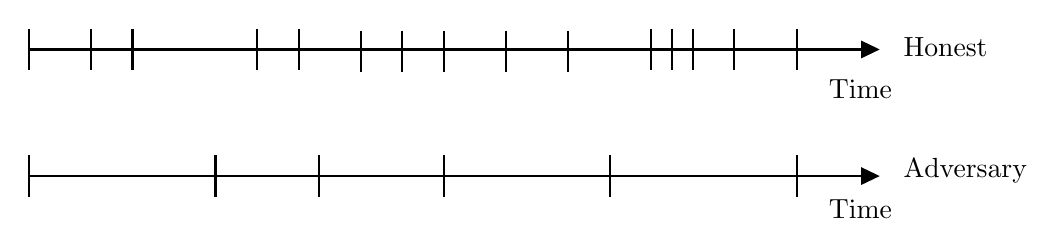
\begin{tikzpicture}[x=0.75pt,y=0.75pt,yscale=-1,xscale=1]
%uncomment if require: \path (0,112); %set diagram left start at 0, and has height of 112

%Straight Lines [id:da23525023892191266]
\draw    (140,20) -- (547,20) ;
\draw [shift={(550,20)}, rotate = 180] [fill={rgb, 255:red, 0; green, 0; blue, 0 }  ][line width=0.08]  [draw opacity=0] (8.93,-4.29) -- (0,0) -- (8.93,4.29) -- cycle    ;
%Straight Lines [id:da7960445132740581]
\draw    (140,10) -- (140,30) ;
%Straight Lines [id:da29783337527097675]
\draw    (270,10) -- (270,30) ;
%Straight Lines [id:da33677894078119586]
\draw    (190,10) -- (190,30) ;
%Straight Lines [id:da5399367214918731]
\draw    (370,11) -- (370,31) ;
%Straight Lines [id:da09675758542474289]
\draw    (440,10) -- (440,30) ;
%Straight Lines [id:da5769918595193868]
\draw    (450,10) -- (450,30) ;
%Straight Lines [id:da31319754434895075]
\draw    (460,10) -- (460,30) ;
%Straight Lines [id:da33141985537928864]
\draw    (510,10) -- (510,30) ;
%Straight Lines [id:da11800923635182015]
\draw    (140,81) -- (547,81) ;
\draw [shift={(550,81)}, rotate = 180] [fill={rgb, 255:red, 0; green, 0; blue, 0 }  ][line width=0.08]  [draw opacity=0] (8.93,-4.29) -- (0,0) -- (8.93,4.29) -- cycle    ;
%Straight Lines [id:da07789537672362723]
\draw    (140,71) -- (140,91) ;
%Straight Lines [id:da8372706005219659]
\draw    (280,71) -- (280,91) ;
%Straight Lines [id:da29756814685721467]
\draw    (230,71) -- (230,91) ;
%Straight Lines [id:da86063133847938]
\draw    (340,71) -- (340,91) ;
%Straight Lines [id:da599322584965772]
\draw    (420,71) -- (420,91) ;
%Straight Lines [id:da03302559846585229]
\draw    (510,71) -- (510,91) ;
%Straight Lines [id:da21596375747665641]
\draw    (340,11) -- (340,31) ;
%Straight Lines [id:da8449429552182337]
\draw    (320,11) -- (320,31) ;
%Straight Lines [id:da022987682318881708]
\draw    (250,10) -- (250,30) ;
%Straight Lines [id:da9209115770539547]
\draw    (170,10) -- (170,30) ;
%Straight Lines [id:da03134967763740537]
\draw    (300,11) -- (300,31) ;
%Straight Lines [id:da8935379151898348]
\draw    (400,11) -- (400,31) ;
%Straight Lines [id:da957853887353433]
\draw    (480,10) -- (480,30) ;

% Text Node
\draw (524,33) node [anchor=north west][inner sep=0.75pt]   [align=left] {Time};
% Text Node
\draw (560,13) node [anchor=north west][inner sep=0.75pt]   [align=left] {Honest};
% Text Node
\draw (524,91) node [anchor=north west][inner sep=0.75pt]   [align=left] {Time};
% Text Node
\draw (560,71) node [anchor=north west][inner sep=0.75pt]   [align=left] {Adversary};


\end{tikzpicture}
    \caption{Block production of honest nodes vs. the adversary}
    \label{fig:Honest block production power}
\end{figure}

\begin{figure}[H]
	\centering
\tikzset{every picture/.style={line width=0.75pt}} %set default line width to 0.75pt

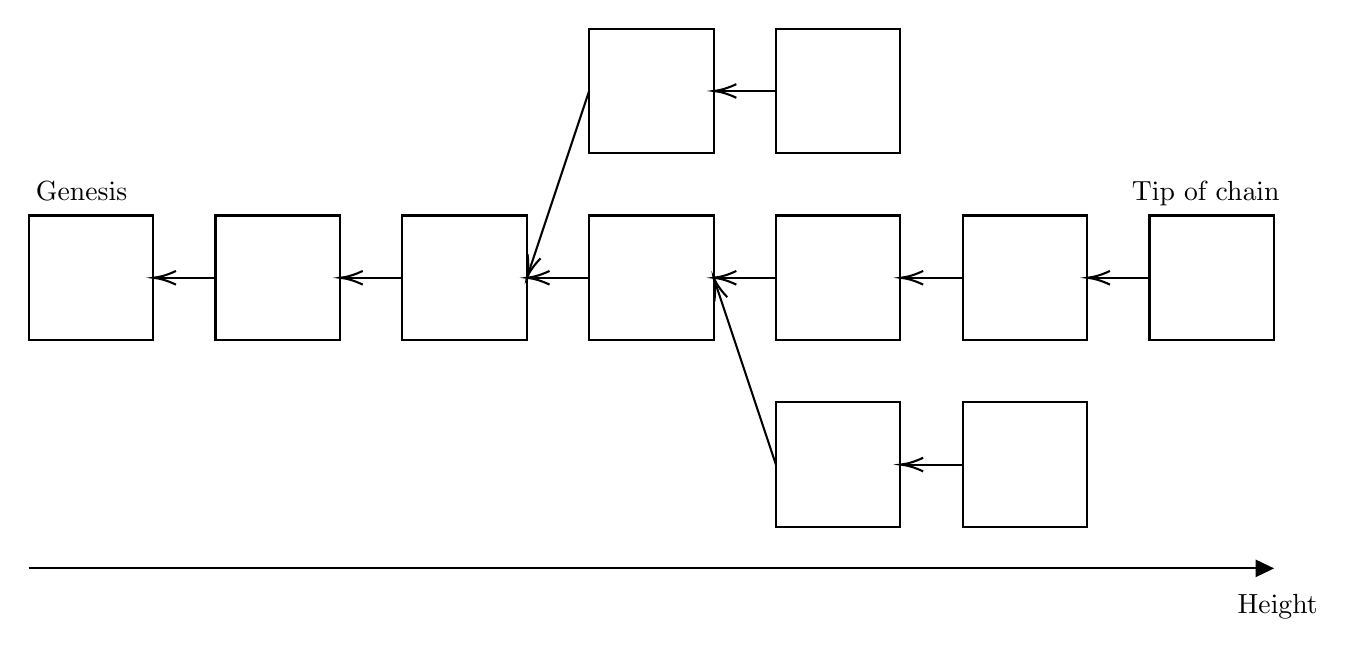
\begin{tikzpicture}[x=0.75pt,y=0.75pt,yscale=-1,xscale=1]
%uncomment if require: \path (0,317); %set diagram left start at 0, and has height of 317

%Shape: Square [id:dp5553489928334188]
\draw   (20,100) -- (80,100) -- (80,160) -- (20,160) -- cycle ;
%Straight Lines [id:da02867875054034763]
\draw    (110,130) -- (82,130) ;
\draw [shift={(80,130)}, rotate = 360] [color={rgb, 255:red, 0; green, 0; blue, 0 }  ][line width=0.75]    (10.93,-3.29) .. controls (6.95,-1.4) and (3.31,-0.3) .. (0,0) .. controls (3.31,0.3) and (6.95,1.4) .. (10.93,3.29)   ;
%Shape: Square [id:dp49650358706771236]
\draw   (110,100) -- (170,100) -- (170,160) -- (110,160) -- cycle ;
%Straight Lines [id:da05327516325435977]
\draw    (200,130) -- (172,130) ;
\draw [shift={(170,130)}, rotate = 360] [color={rgb, 255:red, 0; green, 0; blue, 0 }  ][line width=0.75]    (10.93,-3.29) .. controls (6.95,-1.4) and (3.31,-0.3) .. (0,0) .. controls (3.31,0.3) and (6.95,1.4) .. (10.93,3.29)   ;
%Shape: Square [id:dp44489240803143804]
\draw   (200,100) -- (260,100) -- (260,160) -- (200,160) -- cycle ;
%Straight Lines [id:da7431038331619342]
\draw    (290,130) -- (262,130) ;
\draw [shift={(260,130)}, rotate = 360] [color={rgb, 255:red, 0; green, 0; blue, 0 }  ][line width=0.75]    (10.93,-3.29) .. controls (6.95,-1.4) and (3.31,-0.3) .. (0,0) .. controls (3.31,0.3) and (6.95,1.4) .. (10.93,3.29)   ;
%Shape: Square [id:dp540021094447644]
\draw   (290,100) -- (350,100) -- (350,160) -- (290,160) -- cycle ;
%Shape: Square [id:dp86801051079086]
\draw   (380,190) -- (440,190) -- (440,250) -- (380,250) -- cycle ;
%Straight Lines [id:da6968247771293123]
\draw    (380,220) -- (350.63,131.9) ;
\draw [shift={(350,130)}, rotate = 71.57] [color={rgb, 255:red, 0; green, 0; blue, 0 }  ][line width=0.75]    (10.93,-3.29) .. controls (6.95,-1.4) and (3.31,-0.3) .. (0,0) .. controls (3.31,0.3) and (6.95,1.4) .. (10.93,3.29)   ;
%Straight Lines [id:da10617452462704291]
\draw    (470,220) -- (442,220) ;
\draw [shift={(440,220)}, rotate = 360] [color={rgb, 255:red, 0; green, 0; blue, 0 }  ][line width=0.75]    (10.93,-3.29) .. controls (6.95,-1.4) and (3.31,-0.3) .. (0,0) .. controls (3.31,0.3) and (6.95,1.4) .. (10.93,3.29)   ;
%Shape: Square [id:dp013136466066319574]
\draw   (470,190) -- (530,190) -- (530,250) -- (470,250) -- cycle ;
%Straight Lines [id:da5171350092317244]
\draw    (380,130) -- (352,130) ;
\draw [shift={(350,130)}, rotate = 360] [color={rgb, 255:red, 0; green, 0; blue, 0 }  ][line width=0.75]    (10.93,-3.29) .. controls (6.95,-1.4) and (3.31,-0.3) .. (0,0) .. controls (3.31,0.3) and (6.95,1.4) .. (10.93,3.29)   ;
%Shape: Square [id:dp6846062105068249]
\draw   (380,100) -- (440,100) -- (440,160) -- (380,160) -- cycle ;
%Shape: Square [id:dp863890663182566]
\draw   (290,10) -- (350,10) -- (350,70) -- (290,70) -- cycle ;
%Straight Lines [id:da04868739915580034]
\draw    (290,40) -- (260.63,128.1) ;
\draw [shift={(260,130)}, rotate = 288.43] [color={rgb, 255:red, 0; green, 0; blue, 0 }  ][line width=0.75]    (10.93,-3.29) .. controls (6.95,-1.4) and (3.31,-0.3) .. (0,0) .. controls (3.31,0.3) and (6.95,1.4) .. (10.93,3.29)   ;
%Straight Lines [id:da36373788691107434]
\draw    (380,40) -- (352,40) ;
\draw [shift={(350,40)}, rotate = 360] [color={rgb, 255:red, 0; green, 0; blue, 0 }  ][line width=0.75]    (10.93,-3.29) .. controls (6.95,-1.4) and (3.31,-0.3) .. (0,0) .. controls (3.31,0.3) and (6.95,1.4) .. (10.93,3.29)   ;
%Shape: Square [id:dp8457049773626129]
\draw   (380,10) -- (440,10) -- (440,70) -- (380,70) -- cycle ;
%Shape: Square [id:dp746865970815856]
\draw   (470,100) -- (530,100) -- (530,160) -- (470,160) -- cycle ;
%Straight Lines [id:da7437715956006345]
\draw    (560,130) -- (532,130) ;
\draw [shift={(530,130)}, rotate = 360] [color={rgb, 255:red, 0; green, 0; blue, 0 }  ][line width=0.75]    (10.93,-3.29) .. controls (6.95,-1.4) and (3.31,-0.3) .. (0,0) .. controls (3.31,0.3) and (6.95,1.4) .. (10.93,3.29)   ;
%Shape: Square [id:dp9434239793653232]
\draw   (560,100) -- (620,100) -- (620,160) -- (560,160) -- cycle ;
%Straight Lines [id:da06385468421590201]
\draw    (470,130) -- (442,130) ;
\draw [shift={(440,130)}, rotate = 360] [color={rgb, 255:red, 0; green, 0; blue, 0 }  ][line width=0.75]    (10.93,-3.29) .. controls (6.95,-1.4) and (3.31,-0.3) .. (0,0) .. controls (3.31,0.3) and (6.95,1.4) .. (10.93,3.29)   ;
%Straight Lines [id:da4081512417331501]
\draw    (20,270) -- (617,270) ;
\draw [shift={(620,270)}, rotate = 180] [fill={rgb, 255:red, 0; green, 0; blue, 0 }  ][line width=0.08]  [draw opacity=0] (8.93,-4.29) -- (0,0) -- (8.93,4.29) -- cycle    ;
%Straight Lines [id:da6329335012714348]
% \draw    (20,260) -- (20,280) ;
%Straight Lines [id:da5452663697779279]
% \draw    (110,260) -- (110,280) ;
%Straight Lines [id:da8605249971113638]
% \draw    (200,260) -- (200,280) ;
%Straight Lines [id:da8480595218681781]
% \draw    (290,260) -- (290,280) ;
%Straight Lines [id:da13016480179291512]
% \draw    (380,260) -- (380,280) ;
%Straight Lines [id:da0032258538987217644]
% \draw    (470,260) -- (470,280) ;
%Straight Lines [id:da08791748462517157]
% \draw    (560,260) -- (560,280) ;

% Text Node
\draw (550,82) node [anchor=north west][inner sep=0.75pt]   [align=left] {Tip of chain};
% Text Node
\draw (601,281) node [anchor=north west][inner sep=0.75pt]   [align=left] {Height};
% Text Node
\draw (22,82) node [anchor=north west][inner sep=0.75pt]   [align=left] {Genesis};
% Text Node
% \draw (15,282.4) node [anchor=north west][inner sep=0.75pt]    {$0$};
% % Text Node
% \draw (105,282.4) node [anchor=north west][inner sep=0.75pt]    {$1$};
% % Text Node
% \draw (195,282.4) node [anchor=north west][inner sep=0.75pt]    {$2$};
% % Text Node
% \draw (285,283.4) node [anchor=north west][inner sep=0.75pt]    {$3$};
% % Text Node
% \draw (375,282.4) node [anchor=north west][inner sep=0.75pt]    {$4$};
% % Text Node
% \draw (465,282.4) node [anchor=north west][inner sep=0.75pt]    {$5$};
% % Text Node
% \draw (555,282.4) node [anchor=north west][inner sep=0.75pt]    {$6$};


\end{tikzpicture}
	\caption{Block trees and the longest chain rule. There may be temporary forks because of conflicting blocks. But, the occurrence of convergence opportunities ensures that eventually, there will be a unique tip of the longest chain.}
	\label{fig:Block tree}  %Tag for referring to figure in text.
\end{figure}

\section{Coinbase Transactions}

While we have successfully implemented a way to validate ownership of money in a decentralized manner, we have yet to see how to tackle the creation of money.

To do so, we introduce the notion of a ``coinbase transaction''. This transaction is uniquely present in every block. The miner creates this transaction, and can reward any public key they want with an amount less than or equal to a fixed amount $f$ (the block reward) determined by the network plus transaction fees (the fee reward). These fees correspond to the difference between inputs and outputs in each transaction confirmed in the block. Due to the weak law of conservation, recall that there can be a difference between the sum of the inputs and the sum of the outputs in each transaction. This difference is paid out as fees. In other words, the miner can create a transaction with no input and one output with an amount $a$ respecting the following equation:
\begin{equation}
    a \leq f + \sum_{i \in {\text{input}}} i.v - \sum_{o \in {\text{ouput}}} o.v
\end{equation}
where the sum is over all transactions in the block.
In our Marabu protocol, we use $f = 50$ bu.

Finally, to avoid multiple identical transactions that would have the same hash as a result of having the same amount and same public key output, an additional \emph{height} parameter is included in the coinbase transaction. This parameter corresponds to the number of blocks that this block is away from genesis.

\section{Verifying Objects}

\subsection{Verifying a Block}

Upon receiving a block, a honest node should:
\begin{enumerate}
    \item Verify the proof of work (and do this first to avoid spam attacks).
    \item Verify the parent block recursively (and if it does not exist locally, request it from the network).
    \item Verify the transactions inside the block, including the coinbase transaction (and if it does not have them, request them from the network).
\end{enumerate}

\subsection{Verifying a Chain}

Upon receiving a chain, a honest node should:
\begin{enumerate}
    \item Verify each block in the chain.
    \item Check that it starts with genesis (or is connected to a block known to be connected to genesis).
    \item Adopt the longest chain or one of the longest chains.
\end{enumerate}

\subsection{Verifying a Regular Transaction}

See lecture 4

\subsection{Verifying a Coinbase Transaction}

A valid coinbase transaction must:
\begin{enumerate}
    \item be the only one in that block,
    \item be the first transaction in the block,
    \item have no input and exactly one output,
    \item have a value which is less than or equal to the sum of the fixed block reward and the difference between the input and output amounts of all other transactions in the block,
    \item not be spent in the same block.
\end{enumerate}

\section{Comparing Transactions and Blocks}

Now that we understand how blocks and transactions work, it is worth drawing parallels between the two.
\begin{center}
\begin{tabular}{ |c|c|c| }
  \hline
  & \textbf{Transaction} & \textbf{Block} \\
  \hline
  \textbf{Inductive base} & Coinbase & Genesis \\
  \hline
  \textbf{Inductive hypothesis} & Outpoint UTXO & Previous ID ($s$) \\
  \hline
  \textbf{Inductive step} & \makecell{Consuming produced UTXO \\ Signatures \\ Conservation laws} & \makecell{Proof of Work \\ Causality \\ Transactions} \\
  \hline
\end{tabular}
\end{center}

\section{Updating the UTXO}

For each received transaction, if the transaction is valid, apply the transaction to the previous UTXO to get the new UTXO.

For each reveived block, apply each transaction of the block to the previous UTXO. If at any point a transaction is invalid, reject the entire block and revert to the previous UTXO.

For all transactions not yet in a block, add them to a mempool with a temporary UTXO which starts as the same UTXO as the current longest chain tip. These transactions are added in the order in which they are received. If the transaction is invalid with respect to the current UTXO, reject it. When mining a block, use all of the transactions in the mempool to create this block.

Upon receiving a block at the tip of the current longest chain, validate the block and update the UTXO. Also update the mempool and temporary UTXO by applying transactions in the block or removing any transaction that is now either invalid or already in the newly received block.

Upon receiving a block which changes the longest chain to another chain, set the UTXO to the fork between the current longest chain and this new chain (by undoing all transactions after the fork in the current chain). Then, go through each block until the tip in the new longest chain and update the UTXO. If at any point, a block is invalid, reject the new chain and revert to the previous chain and previous UTXO. If all blocks after the fork in the new longest chain are valid, update the mempool by starting with the UTXO at the tip of the new longest chain, applying every valid transaction in the previous longest chain that is not present in the new longest chain, then applying all the still-valid transactions that were previously in the mempool. This process of adopting the longest chain is shown in Figure~\ref{fig:UTXOChainChange}. \\

\begin{figure}[H]
    \centering
\tikzset{every picture/.style={line width=0.75pt}} %set default line width to 0.75pt

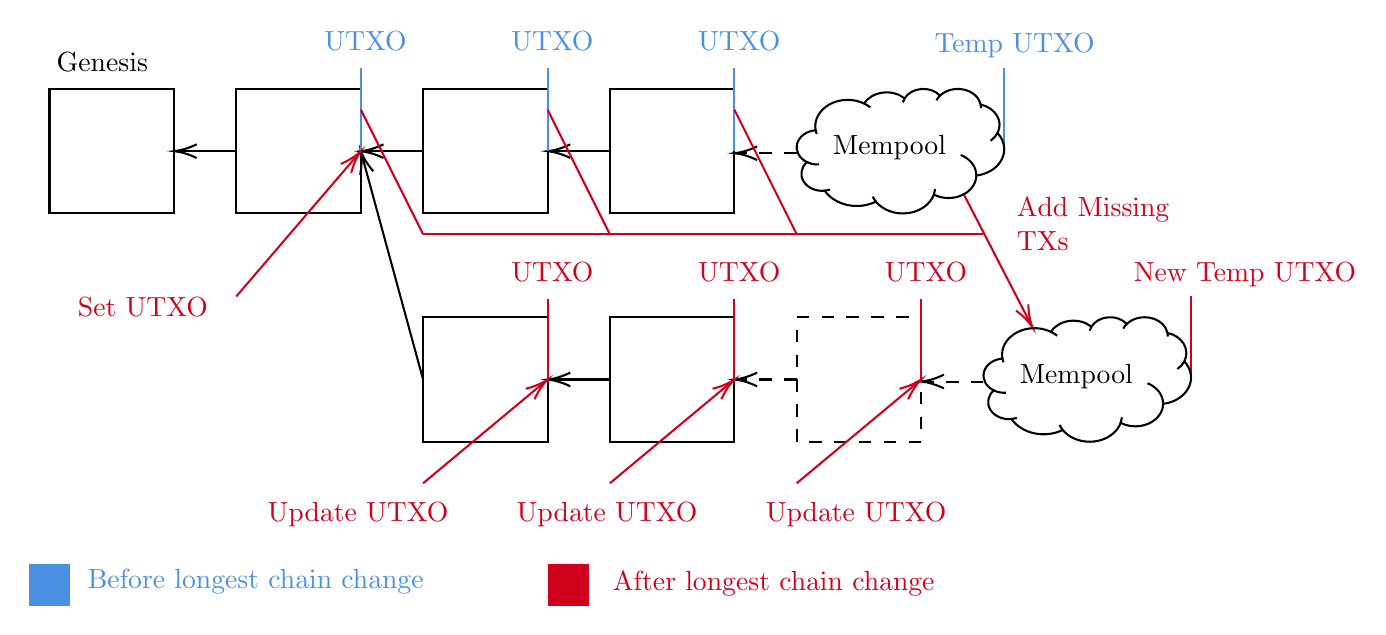
\begin{tikzpicture}[x=0.75pt,y=0.75pt,yscale=-1,xscale=1]
%uncomment if require: \path (0,303); %set diagram left start at 0, and has height of 303

%Shape: Square [id:dp6521466830611065]
\draw   (20,41) -- (80,41) -- (80,101) -- (20,101) -- cycle ;
%Straight Lines [id:da7819102316771764]
\draw    (110,71) -- (82,71) ;
\draw [shift={(80,71)}, rotate = 360] [color={rgb, 255:red, 0; green, 0; blue, 0 }  ][line width=0.75]    (10.93,-3.29) .. controls (6.95,-1.4) and (3.31,-0.3) .. (0,0) .. controls (3.31,0.3) and (6.95,1.4) .. (10.93,3.29)   ;
%Shape: Square [id:dp6182477130409076]
\draw   (110,41) -- (170,41) -- (170,101) -- (110,101) -- cycle ;
%Straight Lines [id:da22654224529120404]
\draw    (200,71) -- (172,71) ;
\draw [shift={(170,71)}, rotate = 360] [color={rgb, 255:red, 0; green, 0; blue, 0 }  ][line width=0.75]    (10.93,-3.29) .. controls (6.95,-1.4) and (3.31,-0.3) .. (0,0) .. controls (3.31,0.3) and (6.95,1.4) .. (10.93,3.29)   ;
%Shape: Square [id:dp02337826181900904]
\draw   (200,41) -- (260,41) -- (260,101) -- (200,101) -- cycle ;
%Straight Lines [id:da15734675441574208]
\draw    (290,71) -- (262,71) ;
\draw [shift={(260,71)}, rotate = 360] [color={rgb, 255:red, 0; green, 0; blue, 0 }  ][line width=0.75]    (10.93,-3.29) .. controls (6.95,-1.4) and (3.31,-0.3) .. (0,0) .. controls (3.31,0.3) and (6.95,1.4) .. (10.93,3.29)   ;
%Shape: Square [id:dp840092006051874]
\draw   (290,41) -- (350,41) -- (350,101) -- (290,101) -- cycle ;
%Shape: Square [id:dp801014946422226]
\draw   (200,151) -- (260,151) -- (260,211) -- (200,211) -- cycle ;
%Straight Lines [id:da9537380349189299]
\draw    (200,181) -- (170.53,72.93) ;
\draw [shift={(170,71)}, rotate = 74.74] [color={rgb, 255:red, 0; green, 0; blue, 0 }  ][line width=0.75]    (10.93,-3.29) .. controls (6.95,-1.4) and (3.31,-0.3) .. (0,0) .. controls (3.31,0.3) and (6.95,1.4) .. (10.93,3.29)   ;
%Straight Lines [id:da8212782642294261]
\draw    (290,181) -- (262,181) ;
\draw [shift={(260,181)}, rotate = 360] [color={rgb, 255:red, 0; green, 0; blue, 0 }  ][line width=0.75]    (10.93,-3.29) .. controls (6.95,-1.4) and (3.31,-0.3) .. (0,0) .. controls (3.31,0.3) and (6.95,1.4) .. (10.93,3.29)   ;
%Shape: Square [id:dp22084257855473166]
\draw   (290,151) -- (350,151) -- (350,211) -- (290,211) -- cycle ;
%Straight Lines [id:da9533389147995392]
\draw  [dash pattern={on 4.5pt off 4.5pt}]  (380,181) -- (352,181) ;
\draw [shift={(350,181)}, rotate = 360] [color={rgb, 255:red, 0; green, 0; blue, 0 }  ][line width=0.75]    (10.93,-3.29) .. controls (6.95,-1.4) and (3.31,-0.3) .. (0,0) .. controls (3.31,0.3) and (6.95,1.4) .. (10.93,3.29)   ;
%Shape: Square [id:dp9382911344304163]
\draw  [dash pattern={on 4.5pt off 4.5pt}] (380,151) -- (440,151) -- (440,211) -- (380,211) -- cycle ;
%Straight Lines [id:da7513116931470782]
\draw [color={rgb, 255:red, 74; green, 144; blue, 226 }  ,draw opacity=1 ]   (170,31) -- (170,71) ;
%Straight Lines [id:da7430295277757613]
\draw [color={rgb, 255:red, 74; green, 144; blue, 226 }  ,draw opacity=1 ]   (260,31) -- (260,71) ;
%Straight Lines [id:da11052295583016747]
\draw [color={rgb, 255:red, 74; green, 144; blue, 226 }  ,draw opacity=1 ]   (350,31) -- (350,71) ;
%Straight Lines [id:da8715298181677615]
\draw [color={rgb, 255:red, 208; green, 2; blue, 27 }  ,draw opacity=1 ]   (260,142) -- (260,182) ;
%Straight Lines [id:da9627172266750117]
\draw [color={rgb, 255:red, 208; green, 2; blue, 27 }  ,draw opacity=1 ]   (350,142) -- (350,182) ;
%Straight Lines [id:da3023883615554328]
\draw [color={rgb, 255:red, 208; green, 2; blue, 27 }  ,draw opacity=1 ]   (110,141) -- (168.7,72.52) ;
\draw [shift={(170,71)}, rotate = 130.6] [color={rgb, 255:red, 208; green, 2; blue, 27 }  ,draw opacity=1 ][line width=0.75]    (10.93,-3.29) .. controls (6.95,-1.4) and (3.31,-0.3) .. (0,0) .. controls (3.31,0.3) and (6.95,1.4) .. (10.93,3.29)   ;
%Straight Lines [id:da9901888064889268]
\draw [color={rgb, 255:red, 208; green, 2; blue, 27 }  ,draw opacity=1 ]   (200,231) -- (214.92,218.57) -- (258.46,182.28) ;
\draw [shift={(260,181)}, rotate = 140.19] [color={rgb, 255:red, 208; green, 2; blue, 27 }  ,draw opacity=1 ][line width=0.75]    (10.93,-3.29) .. controls (6.95,-1.4) and (3.31,-0.3) .. (0,0) .. controls (3.31,0.3) and (6.95,1.4) .. (10.93,3.29)   ;
%Straight Lines [id:da7470962668798595]
\draw [color={rgb, 255:red, 208; green, 2; blue, 27 }  ,draw opacity=1 ]   (440,142) -- (440,182) ;
%Straight Lines [id:da5600163205713113]
\draw [color={rgb, 255:red, 208; green, 2; blue, 27 }  ,draw opacity=1 ]   (460.25,91.25) -- (492.75,154.22) ;
\draw [shift={(493.67,156)}, rotate = 242.7] [color={rgb, 255:red, 208; green, 2; blue, 27 }  ,draw opacity=1 ][line width=0.75]    (10.93,-3.29) .. controls (6.95,-1.4) and (3.31,-0.3) .. (0,0) .. controls (3.31,0.3) and (6.95,1.4) .. (10.93,3.29)   ;
%Straight Lines [id:da535323812611922]
\draw  [dash pattern={on 4.5pt off 4.5pt}]  (380,71.99) -- (352,71.99) ;
\draw [shift={(350,71.99)}, rotate = 360] [color={rgb, 255:red, 0; green, 0; blue, 0 }  ][line width=0.75]    (10.93,-3.29) .. controls (6.95,-1.4) and (3.31,-0.3) .. (0,0) .. controls (3.31,0.3) and (6.95,1.4) .. (10.93,3.29)   ;
%Straight Lines [id:da10474572702800766]
\draw  [dash pattern={on 4.5pt off 4.5pt}]  (470,181.99) -- (442,181.99) ;
\draw [shift={(440,181.99)}, rotate = 360] [color={rgb, 255:red, 0; green, 0; blue, 0 }  ][line width=0.75]    (10.93,-3.29) .. controls (6.95,-1.4) and (3.31,-0.3) .. (0,0) .. controls (3.31,0.3) and (6.95,1.4) .. (10.93,3.29)   ;
%Straight Lines [id:da98694418087908]
\draw [color={rgb, 255:red, 208; green, 2; blue, 27 }  ,draw opacity=1 ]   (170,51) -- (200,111) ;
%Straight Lines [id:da7736807885577637]
\draw [color={rgb, 255:red, 208; green, 2; blue, 27 }  ,draw opacity=1 ]   (260,51) -- (290,111) ;
%Straight Lines [id:da5079296287543524]
\draw [color={rgb, 255:red, 208; green, 2; blue, 27 }  ,draw opacity=1 ]   (350,51) -- (380,111) ;
%Straight Lines [id:da970296926623833]
\draw [color={rgb, 255:red, 208; green, 2; blue, 27 }  ,draw opacity=1 ]   (200,111) -- (470,111) ;
%Straight Lines [id:da16682911027696634]
\draw [color={rgb, 255:red, 74; green, 144; blue, 226 }  ,draw opacity=1 ]   (480,31) -- (480,71) ;
%Straight Lines [id:da9543785277219905]
\draw [color={rgb, 255:red, 208; green, 2; blue, 27 }  ,draw opacity=1 ]   (570,141) -- (570,181) ;
%Shape: Cloud [id:dp30012303953626596]
\draw   (389.1,60.75) .. controls (388.29,55.92) and (390.94,51.13) .. (395.91,48.42) .. controls (400.88,45.71) and (407.31,45.56) .. (412.46,48.03) .. controls (414.29,45.21) and (417.63,43.27) .. (421.48,42.79) .. controls (425.32,42.3) and (429.22,43.33) .. (432,45.57) .. controls (433.55,43.02) and (436.61,41.31) .. (440.08,41.04) .. controls (443.55,40.77) and (446.94,41.98) .. (449.05,44.25) .. controls (451.86,41.55) and (456.33,40.41) .. (460.53,41.33) .. controls (464.73,42.25) and (467.9,45.06) .. (468.67,48.55) .. controls (472.11,49.31) and (474.98,51.27) .. (476.53,53.9) .. controls (478.08,56.53) and (478.16,59.58) .. (476.76,62.27) .. controls (480.15,65.88) and (480.94,70.68) .. (478.84,74.89) .. controls (476.74,79.11) and (472.06,82.09) .. (466.55,82.74) .. controls (466.51,86.69) and (463.86,90.32) .. (459.62,92.22) .. controls (455.38,94.12) and (450.21,94.01) .. (446.1,91.91) .. controls (444.35,96.65) and (439.43,100.13) .. (433.46,100.86) .. controls (427.48,101.59) and (421.54,99.43) .. (418.18,95.32) .. controls (414.07,97.34) and (409.14,97.93) .. (404.49,96.94) .. controls (399.85,95.95) and (395.89,93.46) .. (393.5,90.05) .. controls (389.3,90.45) and (385.24,88.67) .. (383.33,85.59) .. controls (381.42,82.51) and (382.08,78.79) .. (384.97,76.27) .. controls (381.22,74.47) and (379.31,70.89) .. (380.23,67.4) .. controls (381.15,63.92) and (384.69,61.31) .. (389.02,60.94) ; \draw   (384.97,76.27) .. controls (386.74,77.13) and (388.78,77.51) .. (390.83,77.38)(393.5,90.05) .. controls (394.38,89.96) and (395.24,89.79) .. (396.07,89.52)(418.18,95.32) .. controls (417.56,94.56) and (417.05,93.75) .. (416.64,92.9)(446.1,91.91) .. controls (446.42,91.05) and (446.62,90.16) .. (446.72,89.26)(466.55,82.74) .. controls (466.59,78.53) and (463.67,74.67) .. (459.04,72.83)(476.76,62.27) .. controls (476.01,63.7) and (474.86,64.97) .. (473.41,65.98)(468.67,48.55) .. controls (468.79,49.12) and (468.85,49.71) .. (468.84,50.3)(449.05,44.25) .. controls (448.35,44.92) and (447.77,45.68) .. (447.34,46.49)(432,45.57) .. controls (431.62,46.18) and (431.34,46.83) .. (431.17,47.5)(412.46,48.03) .. controls (413.55,48.55) and (414.56,49.18) .. (415.46,49.9)(389.1,60.75) .. controls (389.21,61.42) and (389.39,62.08) .. (389.62,62.72) ;
%Shape: Cloud [id:dp9947625990800526]
\draw   (479.1,170.75) .. controls (478.29,165.92) and (480.94,161.13) .. (485.91,158.42) .. controls (490.88,155.71) and (497.31,155.56) .. (502.46,158.03) .. controls (504.29,155.21) and (507.63,153.27) .. (511.48,152.79) .. controls (515.32,152.3) and (519.22,153.33) .. (522,155.57) .. controls (523.55,153.02) and (526.61,151.31) .. (530.08,151.04) .. controls (533.55,150.77) and (536.94,151.98) .. (539.05,154.25) .. controls (541.86,151.55) and (546.33,150.41) .. (550.53,151.33) .. controls (554.73,152.25) and (557.9,155.06) .. (558.67,158.55) .. controls (562.11,159.31) and (564.98,161.27) .. (566.53,163.9) .. controls (568.08,166.53) and (568.16,169.58) .. (566.76,172.27) .. controls (570.15,175.88) and (570.94,180.68) .. (568.84,184.89) .. controls (566.74,189.11) and (562.06,192.09) .. (556.55,192.74) .. controls (556.51,196.69) and (553.86,200.32) .. (549.62,202.22) .. controls (545.38,204.12) and (540.21,204.01) .. (536.1,201.91) .. controls (534.35,206.65) and (529.43,210.13) .. (523.46,210.86) .. controls (517.48,211.59) and (511.54,209.43) .. (508.18,205.32) .. controls (504.07,207.34) and (499.14,207.93) .. (494.49,206.94) .. controls (489.85,205.95) and (485.89,203.46) .. (483.5,200.05) .. controls (479.3,200.45) and (475.24,198.67) .. (473.33,195.59) .. controls (471.42,192.51) and (472.08,188.79) .. (474.97,186.27) .. controls (471.22,184.47) and (469.31,180.89) .. (470.23,177.4) .. controls (471.15,173.92) and (474.69,171.31) .. (479.02,170.94) ; \draw   (474.97,186.27) .. controls (476.74,187.13) and (478.78,187.51) .. (480.83,187.38)(483.5,200.05) .. controls (484.38,199.96) and (485.24,199.79) .. (486.07,199.52)(508.18,205.32) .. controls (507.56,204.56) and (507.05,203.75) .. (506.64,202.9)(536.1,201.91) .. controls (536.42,201.05) and (536.62,200.16) .. (536.72,199.26)(556.55,192.74) .. controls (556.59,188.53) and (553.67,184.67) .. (549.04,182.83)(566.76,172.27) .. controls (566.01,173.7) and (564.86,174.97) .. (563.41,175.98)(558.67,158.55) .. controls (558.79,159.12) and (558.85,159.71) .. (558.84,160.3)(539.05,154.25) .. controls (538.35,154.92) and (537.77,155.68) .. (537.34,156.49)(522,155.57) .. controls (521.62,156.18) and (521.34,156.83) .. (521.17,157.5)(502.46,158.03) .. controls (503.55,158.55) and (504.56,159.18) .. (505.46,159.9)(479.1,170.75) .. controls (479.21,171.42) and (479.39,172.08) .. (479.62,172.72) ;
%Straight Lines [id:da21490206379605126]
\draw [color={rgb, 255:red, 208; green, 2; blue, 27 }  ,draw opacity=1 ]   (290,231) -- (304.92,218.57) -- (348.46,182.28) ;
\draw [shift={(350,181)}, rotate = 140.19] [color={rgb, 255:red, 208; green, 2; blue, 27 }  ,draw opacity=1 ][line width=0.75]    (10.93,-3.29) .. controls (6.95,-1.4) and (3.31,-0.3) .. (0,0) .. controls (3.31,0.3) and (6.95,1.4) .. (10.93,3.29)   ;
%Straight Lines [id:da21349308780257403]
\draw [color={rgb, 255:red, 208; green, 2; blue, 27 }  ,draw opacity=1 ]   (380,231) -- (394.92,218.57) -- (438.46,182.28) ;
\draw [shift={(440,181)}, rotate = 140.19] [color={rgb, 255:red, 208; green, 2; blue, 27 }  ,draw opacity=1 ][line width=0.75]    (10.93,-3.29) .. controls (6.95,-1.4) and (3.31,-0.3) .. (0,0) .. controls (3.31,0.3) and (6.95,1.4) .. (10.93,3.29)   ;
%Shape: Rectangle [id:dp7810240526075007]
\draw  [draw opacity=0][fill={rgb, 255:red, 208; green, 2; blue, 27 }  ,fill opacity=1 ] (260,270) -- (280,270) -- (280,290) -- (260,290) -- cycle ;
%Shape: Rectangle [id:dp19832461992006012]
\draw  [draw opacity=0][fill={rgb, 255:red, 74; green, 144; blue, 226 }  ,fill opacity=1 ] (10,270) -- (30,270) -- (30,290) -- (10,290) -- cycle ;

% Text Node
\draw (151,12) node [anchor=north west][inner sep=0.75pt]   [align=left] {\textcolor[rgb]{0.29,0.56,0.89}{UTXO}};
% Text Node
\draw (241,12) node [anchor=north west][inner sep=0.75pt]   [align=left] {\textcolor[rgb]{0.29,0.56,0.89}{UTXO}};
% Text Node
\draw (331,12) node [anchor=north west][inner sep=0.75pt]   [align=left] {\textcolor[rgb]{0.29,0.56,0.89}{UTXO}};
% Text Node
\draw (396,62) node [anchor=north west][inner sep=0.75pt]   [align=left] {Mempool};
% Text Node
\draw (241,123) node [anchor=north west][inner sep=0.75pt]  [color={rgb, 255:red, 208; green, 2; blue, 27 }  ,opacity=1 ] [align=left] {\textcolor[rgb]{0.82,0.01,0.11}{UTXO}};
% Text Node
\draw (331,123) node [anchor=north west][inner sep=0.75pt]  [color={rgb, 255:red, 208; green, 2; blue, 27 }  ,opacity=1 ] [align=left] {\textcolor[rgb]{0.82,0.01,0.11}{UTXO}};
% Text Node
\draw (70,146) node  [color={rgb, 255:red, 208; green, 2; blue, 27 }  ,opacity=1 ] [align=left] {\begin{minipage}[lt]{54.4pt}\setlength\topsep{0pt}
Set UTXO
\end{minipage}};
% Text Node
\draw (175,246) node  [color={rgb, 255:red, 208; green, 2; blue, 27 }  ,opacity=1 ] [align=left] {\begin{minipage}[lt]{74.8pt}\setlength\topsep{0pt}
Update UTXO
\end{minipage}};
% Text Node
\draw (421,123) node [anchor=north west][inner sep=0.75pt]  [color={rgb, 255:red, 208; green, 2; blue, 27 }  ,opacity=1 ] [align=left] {\textcolor[rgb]{0.82,0.01,0.11}{UTXO}};
% Text Node
\draw (445,13) node [anchor=north west][inner sep=0.75pt]   [align=left] {\textcolor[rgb]{0.29,0.56,0.89}{Temp UTXO}};
% Text Node
\draw (545,106) node  [color={rgb, 255:red, 208; green, 2; blue, 27 }  ,opacity=1 ] [align=left] {\begin{minipage}[lt]{88.4pt}\setlength\topsep{0pt}
Add Missing\\TXs
\end{minipage}};
% Text Node
\draw (541,123) node [anchor=north west][inner sep=0.75pt]  [color={rgb, 255:red, 208; green, 2; blue, 27 }  ,opacity=1 ] [align=left] {\textcolor[rgb]{0.82,0.01,0.11}{New Temp UTXO}};
% Text Node
\draw (486,172) node [anchor=north west][inner sep=0.75pt]   [align=left] {Mempool};
% Text Node
\draw (290,272) node [anchor=north west][inner sep=0.75pt]  [color={rgb, 255:red, 208; green, 2; blue, 27 }  ,opacity=1 ] [align=left] {After longest chain change};
% Text Node
\draw (295,246) node  [color={rgb, 255:red, 208; green, 2; blue, 27 }  ,opacity=1 ] [align=left] {\begin{minipage}[lt]{74.8pt}\setlength\topsep{0pt}
Update UTXO
\end{minipage}};
% Text Node
\draw (415,246) node  [color={rgb, 255:red, 208; green, 2; blue, 27 }  ,opacity=1 ] [align=left] {\begin{minipage}[lt]{74.8pt}\setlength\topsep{0pt}
Update UTXO
\end{minipage}};
% Text Node
\draw (37,271) node [anchor=north west][inner sep=0.75pt]  [color={rgb, 255:red, 74; green, 144; blue, 226 }  ,opacity=1 ] [align=left] {Before longest chain change};
% Text Node
\draw (22,22) node [anchor=north west][inner sep=0.75pt]   [align=left] {Genesis};


\end{tikzpicture}
    \caption{Updating the UTXO upon chain change: 1. Set UTXO to the fork. 2. Update UTXO by applying blocks in the new chain. 3. Create a new temporary UTXO starting at the tip of the new chain. 4. Add transactions from the previous chain and previous mempool that are missing in the new chain to the new mempool.}
    \label{fig:UTXOChainChange}
\end{figure}

\tikzset{every picture/.style={line width=0.75pt}} %set default line width to 0.75pt
